\RequirePackage[l2tabu, orthodox]{nag}
\documentclass[11pt, a4paper]{report}

\usepackage[utf8]{inputenc}
\usepackage[a4paper]{geometry}
\usepackage{lmodern}
\usepackage{microtype}

% Font stuff:
\usepackage{mathpazo} % Use the Palatino font.
\linespread{1.05}
\usepackage{tgcursor}

\usepackage{xargs}
\usepackage[pdftex, dvipsnames, usenames]{xcolor}
\usepackage[colorinlistoftodos, prependcaption, textsize=tiny]{todonotes}
\usepackage{upquote}
\usepackage{ellipsis}
\usepackage{booktabs}
\usepackage{parskip}
\usepackage{graphicx} % https://en.wikibooks.org/wiki/LaTeX/Importing_Graphics
\usepackage{dirtree}  % Required for directory trees.
\usepackage{listings} % Required for inserting code snippets.
\usepackage{enumitem} % http://tex.stackexchange.com/questions/10684/vertical-space-in-lists
\setlist{itemsep=.1em}
\PassOptionsToPackage{hyphens}{url}
\usepackage[colorlinks=false, pdfborder={0 0 0}, unicode=true]{hyperref}
\urlstyle{same} % don't use monospace font for urls

% Use dash for items in lists:
\renewcommand{\labelitemi}{$-$}
\renewcommand{\labelitemii}{$-$}
\renewcommand{\labelitemiii}{$-$}
\renewcommand{\labelitemiv}{$-$}

% Own syntax highlighting:
% http://www.latextemplates.com/template/code-snippet
% http://www.stud.math.ntnu.no/kurs/latexdocs/listings.pdf
\lstset{
    basicstyle=\ttfamily, % The default font size and style of the code.
    breakatwhitespace=true, % If true, only allows line breaks at white space.
    breaklines=true, % Automatic line breaking (prevents code from protruding outside the box).
    tabsize=2, % Number of spaces per tab in the code
    captionpos=b, % Sets the caption position: b for bottom; t for top
    numbersep=10pt, % Distance of line numbers from the code box.
    numberstyle=\tiny\color{Gray}, % Style used for line numbers.
    firstnumber=1, % Line numbers begin at line 1.
    stepnumber=1, % The step distance between line numbers, i.e. how often will lines be    numbered.
}
\lstdefinelanguage{CayThe}{
    %escapeinside={\%}, % This allows you to escape to LaTeX using the character in the bracket
    keywordstyle=\textbf, 
    morekeywords={group, artifact, version, namespace, import, export, public, package, method},
    sensitive=true,
    numbers=none, % Location of line numbers, can take the values of: none, left, right
    showstringspaces=false, % Don't put marks in string spaces
    showtabs=false, % Display tabs in the code as lines.
    morestring=[b]",
    %stringstyle=\color{Purple}, % Strings are purple.
    morecomment=[l]{//}, 
    morecomment=[s]{/*}{*/},
}

\makeatletter
% Customize the title.
% http://www.latextemplates.com/cat/title-pages
\renewcommand{\maketitle}{\begingroup
    \hbox{
        \hspace*{0.05\textwidth} % Whitespace to the left of the title page.
        \rule{3pt}{\textheight}
        \hspace*{0.07\textwidth} % Whitespace between the vertical line and title page text.
        \parbox[b]{0.95\textwidth}{ % Paragraph box which restricts text to less than the width of the page
            {\noindent\Huge\bfseries\@title\\[0.3\baselineskip] \LARGE Version @(pom.version)}\\[2\baselineskip]
            {\large \textit{\@date}}\\[4\baselineskip] 
            {\Large \textsc{\@author}}

            \vspace{0.5\textheight} % Whitespace between the title block and the publisher
            {\noindent www.weltraumschaf.de}\\[\baselineskip] 
        }
    }
\endgroup}
\makeatother

\title{A Perfect Programming Language}
\author{Sven Strittmatter}
\date{\today}

\begin{document}
\presetkeys{todonotes}{color=blue!20}{}

\maketitle
\thispagestyle{empty}

\tableofcontents

\chapter{Introduction}

\todo{Determine what to add here like: acknowledgement, thanks etc.}

This paper tries to describes what a perfect programming language should constitutes of. We will look at existing programming languages to find what they do well and what are their drawbacks. Then try to describe what such a language must and must not have as features.

\section{Motivation}

What is my motivation behind this: Describe a new perfect programming language? As of time of writing this I have over a decade of experience in programming stuff. I also have experience in various languages: C++, PHP, JavaScript, Ruby, Perl, Java. Also I saw a lot of languages. After some disappointment about the languages I used I started to look around what others do: Go, Python, Erlang, Prolog, Lisp, ML, OCaml, Scala etc.

More and more I saw different languages and their concepts I recognised that most of them have some drawbacks and I started to think about a programming language without any of these. I'm not sure if it is possible to design such a language, but I think it is worth to think about it.

\section{Scope}

This document focus on describing what a perfect programming language should look like, what features it should have and how it should behave. This also includes of course syntax, build tools and dependency management.

But this document does not go into the details, if such a language will be interpreted, compiled or both. Nor it will discuss the execution environment: If it is executed as compiled byte code in a virtual machine, what kind of VM (register or stack based), or as native machine code. All these topics are beyond of the scope of this document. It will describe such a language only from the perspective of the end user: The developer using it to write software.

\chapter{The Good, the Bad and the Ugly}

\todo{Write chapter introduction.}

\section{Drawbacks and Fails}

In this section I'll collect all the drawbacks and fails some already existing languages have. These are not drawbacks only because I say. All of them have some common sense in the community of software craftmanship, clean code developers or others working hard on better software. So the points mentioned here are quite common sense for all well exercised developers. In a later section I will describe ``disappointing'' things which are merely based on my opinion.

\subsection{Null --- The Billion Dollar Fail}

In a lot of programming languages exists a concept of \texttt{null}. This is sometimes called a \textit{null reference} or \textit{null pointer}. Most would have seen such a thing somewhere in their career and have a vague idea what it is: Some not initialised value. Let's have a look what Wikipedia\cite{null-wiki} says what it is:

\begin{quotation}
    In computing, a null pointer has a value reserved for indicating that the pointer does not refer to a valid object. Programs routinely use null pointers to represent conditions such as the end of a list of unknown length or the failure to perform some action; \dots
\end{quotation}

The first thing to mention here is that different languages implement this concept differently. We do not want to dig to deep into these implementation details but concentrate on the perspective of a user of such languages: The problem then arises is the so called \textit{null dereferencing}. From the same Wikipedia\cite{null-wiki} article:

\begin{quotation}
    Because a null pointer does not point to a meaningful object, an attempt to dereference (i.e.\ access the data stored at that memory location) a null pointer usually (but not always) causes a run-time error or immediate program crash.
\end{quotation}

To repeat the crucial part: ``\dots causes a run-time error or immediate program crash.'' To be clear: the problem is not a concept for a not initialised or not present value, rather than dereferencing such will result in program crashes. Lets see some brief examples of such \textit{null dereferences} in various common languages:

\subsubsection{Null in C/C++}
\begin{lstlisting}[language=C++]
    SomeType *obj = nullptr;
    obj->methodCall(); // Crashes the program.
\end{lstlisting}

\subsubsection{Null in Java}
\begin{lstlisting}[language=Java]
    SomeType obj = null;
    name.methodCall(); // Crashes the program.
\end{lstlisting}

\subsubsection{Null in C\#}
\begin{lstlisting}[language={[Sharp]C}]
    SomeType obj = null;
    obj.MethodCall(); // Crashes the program.
\end{lstlisting}

\subsubsection{Null in JavaScript}
In JavaScript there is also \textit{undefined}. It is slightly different than \textit{null}, but this does not matter for the fact that \textit{null dereferences} crashes. Maybe this \textit{undefined} thing is as bad as null too.

\begin{lstlisting}[language=JavaScript]
    var obj = null;
    obj.methodCall(); // Crashes the program.

    obj = {methodCall: null};
    obj.methodCall(); // Crashes the program.
\end{lstlisting}

\subsubsection{Null in PHP}
\begin{lstlisting}[language=PHP]
    $obj = null;
    obj->methodCall(); // Crashes the program.
\end{lstlisting}

\subsubsection{None in Python}
\begin{lstlisting}[language=Python]
    obj = None
    obj.methodCall() # Crashes the program.
\end{lstlisting}

\subsubsection{Nil in Ruby}
\begin{lstlisting}[language=Ruby]
    obj = nil
    obj.method_call # Crashes the program.
\end{lstlisting}

\subsubsection{Null in Perl}
\begin{lstlisting}[language=Perl]
    my $obj;
    $obj->method_call; # Crashes the program.
\end{lstlisting}

All these examples above will compile/translate without any error, but will crash tremendously at runtime. Some might say this is not a problem rather than the concept of the particular language and as a developer you have to deal with such issues: you have to write your program either that you do not produce such \textit{null} values or you deal with them correctly. But this is easier said than done. To paraphrase Murphy's law\cite{murphys-law}: If there is the possibility to make something wrong, then someone will do it wrong at some point in time. As a result developers tend to clutter up code with null checks (called defensive programming). Which will make the code harder to read and reason. As Kent\cite{kent-dyn-err-remediation} stated in his paper \textit{Dynamic Error Remediation: A Case Study with Null Pointer Exceptions}:

\begin{quotation}
    One insidious bug is the null pointer exception, which by its ``null'' nature is hard for programmers to fix. These bugs indicate that nothing was found in memory where something should have been, giving programmers very little to work with to fix the bug besides a stack trace. Null pointer exceptions sometimes show themselves only with certain inputs, making these bugs difficult to find before deployment. \ldots, 1--2\% of developer code is devoted to identifying null objects.
\end{quotation}

Also an important argument is the economic damage done by this kind of bugs. Kent\cite{kent-dyn-err-remediation} cites the NIST that along with developer time and money spent in error checking annually cost of \$59.5 are estimated. From the origin source it is not clear that these costs only came from this kind of bug or from all kinds. Anyway what the real numbers are (it is always difficult to estimate such numbers reliably), the sheer amount mentioned in that paper gives a hint of the the caused damage. This is the same what Tony Hoare\cite{hoare-wiki} the inventor of \textit{null} said later it\cite{hoeare-null} in retrospection:

\begin{quotation}
    I call it my billion-dollar mistake. It was the invention of the null reference in 1965. At that time, I was designing the first comprehensive type system for references in an object oriented language (ALGOL W). My goal was to ensure that all use of references should be absolutely safe, with checking performed automatically by the compiler. But I couldn't resist the temptation to put in a null reference, simply because it was so easy to implement. This has led to innumerable errors, vulnerabilities, and system crashes, which have probably caused a billion dollars of pain and damage in the last forty years.	
\end{quotation} 

Whatever the real economic damage is, the fact that this kind of bug is completely avoidable by removing \textit{null pointers} is obvious. To be clear: There is no problem with the concept that a value may or may not be present. Some languages (as described later) has implemented this without \textit{null pointers}. The problem with \textit{null pointers} is that everything everywhere may be one and either you put lot of checking code into your software or you risk crashes. In statically typed language this also subverts the type system because every type may be null but the statically checking at compile time can't inform you about this problem. As mentioned above the problem will hit reality first at runtime. There are lot of more problems which will be introduced by \textit{null}. A list of some is described by Paul Draper in his blog post \textit{The worst mistake of computer science}\cite{draper-worst-mistake-cs}.

Of course there are techniques to circumvent \textit{null pointer dereferences} in such languages without cluttering up the code with lot of null checks and boiler plate code. You can avoid using null at all. Use empty strings, zero instead of zero, or use \textit{Null Object Pattern}\footnote{\url{https://en.wikipedia.org/wiki/Null_Object_pattern}}. But these are workarounds and introduce the big caveat that a software developer need to know about. Remember yourself starting software development as a novice: You learned about that null thing in your language of choice and of course you used it. Why else should it be part of the language, unless to use it?

Now the interesting question is: \textit{How to deal with values which may or may not be present without introducing null pointers?} Let's look at some languages which try this:

\subsubsection{Nil in Objective-C}
Despite the fact that \textit{Objective-C} has \textit{null} due to its inheritance from C (because it is build on top of C). It has an interesting concept called \texttt{nil}. It is nearly the same as the C \textit{null} (instead of \texttt{(void *)0} it is \texttt{(id)0}). The big difference is that you can send method calls to \textit{nil} without getting an error. The call is simply ignored and returns \textit{nil} as result. So consecutive calls will not fail. This obviates defensive programming as mentioned above. For example a if-expression like

\begin{lstlisting}[language={[Objective]C}]
    if (name != nil && [name isEqualToString:@"Hello, World!"]) {
        ...
    }
\end{lstlisting}

can be simplified to

\begin{lstlisting}[language={[Objective]C}]
    if ([name isEqualToString:@"Hello, World!"]) { 
        ...
    }
\end{lstlisting}

So it is an \textit{opt-in procedure} to ask if a value is \texttt{nil}: In the special case you do not want it you can react on it, but by default the program does not crash. But \textit{Objective-C} has some drawbacks in the field of not initialised references: First it has the C null as mentioned above. This introduces the risk that it is used (if someone didn't know better). Second it is not possible to store \texttt{nil} in collection types and so there is a special container type singleton for that: \texttt{NSNull}. Also there is a distinction between uninitialised object references (\texttt{nil}) and uninitialised class references (\texttt{Nil}). This makes the whole thing complicated and error prone if someone is not familiar with the whole concept.

\subsubsection{Nil in Go}
Go has the philosophy that \textit{value types} should be preferred to pointer types. So a value type will never be \texttt{nil} (which is the Go equivalent for \textit{null}), but a value which has all its properties set to a zero value\cite{golang-spec}. So this example will never fail

\begin{lstlisting}
    var t time.Time
    t.Day()
\end{lstlisting}

But there are no checks if this is done intentionally or if the developer only forgot to call a constructor function. But it will not crash the application because the variable \texttt{t} will be properly initialised to a zeroed value. That means all primitive values such as numbers, booleans, character sequences, collections etc.\ are set to at least a zero equivalent value. Because of the fact that all complex data structures are made of these primitives it is possible to create zeroed values transitively. But as downside it is possible to have an equivalent to a \textit{null pointer dereference}:

\begin{lstlisting}
    var t *time.Timer = nil
    t.Reset(10) // Crashes the program.
\end{lstlisting}

\subsubsection{Nil in Swift}

Nil in Swift is quite similar to Nil in Objective-C:\@

\begin{quotation}
    Optional chaining in Swift is similar to messaging nil in Objective-C, but in a way that works for any type, and that can be checked for success or failure.\cite{swift-spec-optional-chaining}
\end{quotation}

This is done by adding a special operator \texttt{?} for the so called \textit{Optional Chaining}, e.g.

\begin{lstlisting}
    john.residence?.numberOfRooms
\end{lstlisting}

This will not fail if \texttt{residence} is \texttt{nil}. But it introduces the drawback named \textit{Forced Unwrapping}. If the above example is changed to

\begin{lstlisting}
    john.residence!.numberOfRooms
\end{lstlisting}
 and \texttt{residence} is \textit{nil} then the program crashes due to a so called \textit{Forced Unwrapping} of \texttt{nil}:

\begin{quotation}
    The main difference is that optional chaining fails gracefully when the optional is nil, whereas forced unwrapping triggers a runtime error when the optional is nil.\cite{swift-spec-optional-chaining}
\end{quotation}

\subsubsection{Null in F\#}

F\# is a functional language and does not use \textit{null}. This means there is a \textit{null}, but it should not be used. Only for special circumstances:

\begin{quotation}
    The null value is not normally used in F\# for values or variables. However, null appears as an abnormal value in certain situations. If a type is defined in F\#, null is not permitted as a regular value unless the AllowNullLiteral attribute is applied to the type. If a type is defined in some other .NET language, null is a possible value, and when you are interoperating with such types, your F\# code might encounter null values.\cite{null-in-fsharp}
\end{quotation}
 So by default F\# uses the concept of optionals\cite{optional-in-fsharp}. A simple example:

\begin{lstlisting}[language=FSharp]
    let keepIfPositive (a : int) = 
        if a > 0 
        then Some(a) 
        else None
\end{lstlisting}

And checking the presence is done with pattern matching:

\begin{lstlisting}[language=FSharp]
    let exists (x : int option) =
        match x with
        | Some(x) -> true
        | None -> false
\end{lstlisting}

The downside is that \textit{null} may be present due to the fact that in F\# any other .NET language code can be imported. So you can use C\# code and this does have \textit{null} and so F\# must deal with that. This drawback is enforced by the .NET ecosystem in which you can mix the different languages.

\subsubsection{Conclusion}

In general there seems to be nothing wrong to have a concept for representing a \textit{not present value} in a programming language. But as shown above most implementations do this in a problematic way which make it far to easy to introduce bugs in production and will cause an application crash.

I'm not sure which concept is better: Add a \textit{Maybe Type} to the language (like F\# and many other functional languages does) or a \textit{nil} with \textit{Optional Chaining} (like Objective-C or Swift). Anyway which one or a combination would be the best, or any other concept I didn't get yet. There is one major problem all of them have: If you can introduce third party components which have a classical \textit{null}, then this will leak into your component. For example in your language it is possible to link good old C libraries (a lot of languages allow such), then you have to deal with possible \textit{null pointers} (Figure ~\ref{fig:Null_from_linked_native_libs}). 

\begin{figure}[ht]
    \centering
    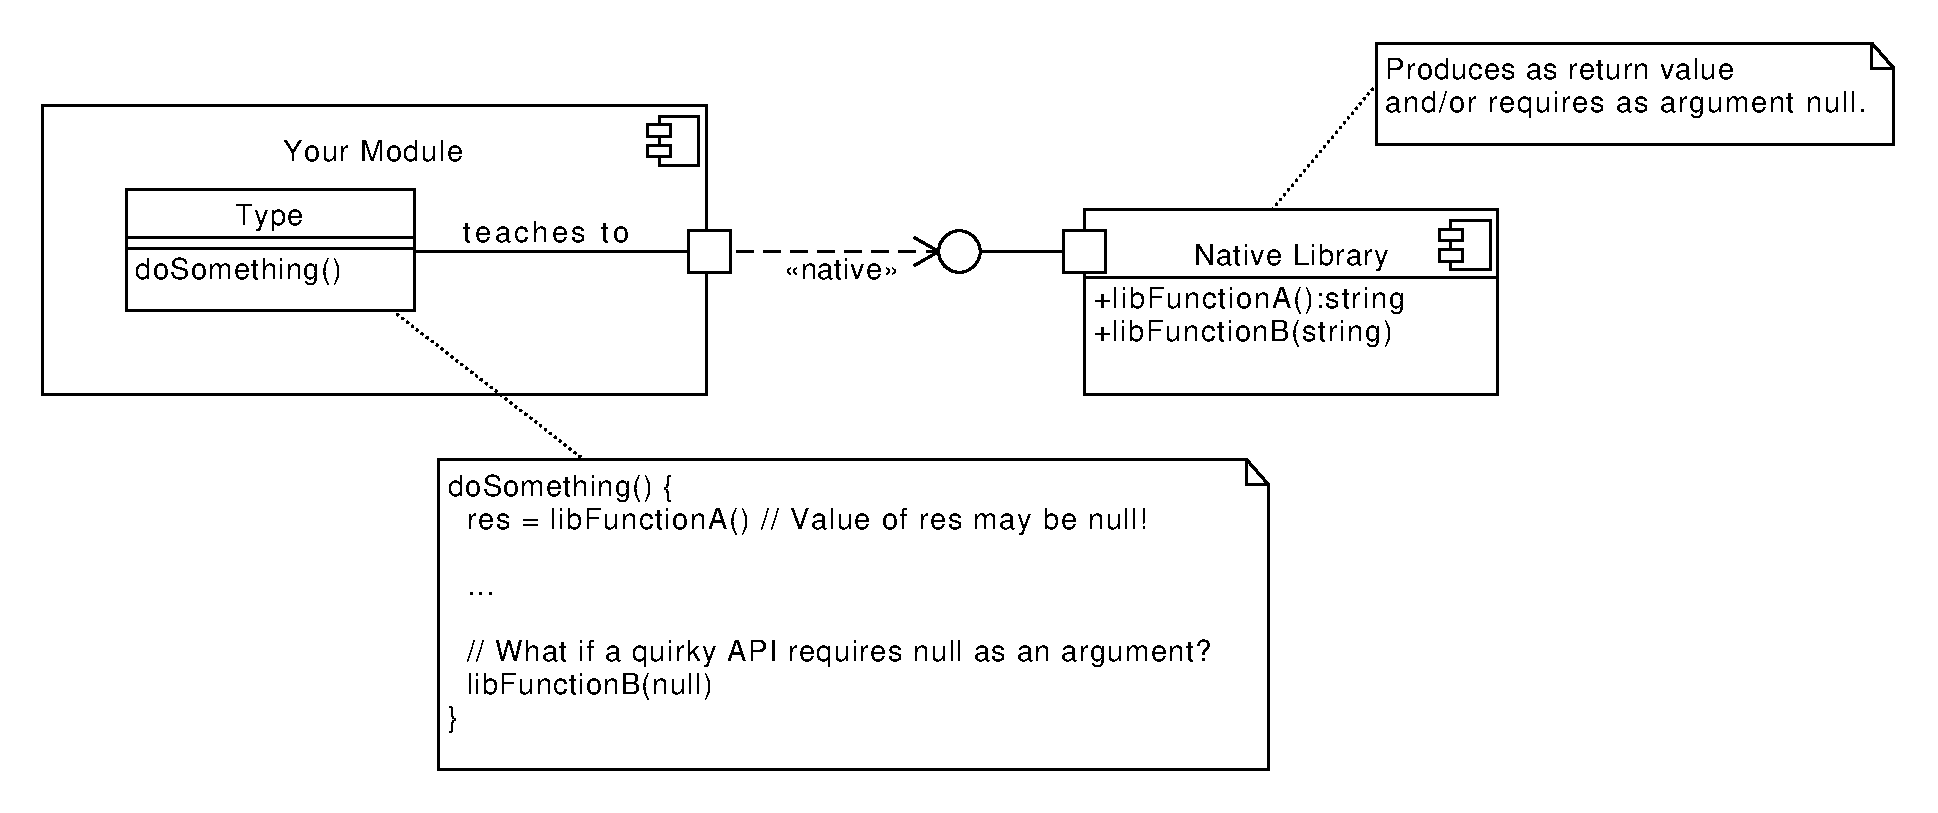
\includegraphics[width=350pt]{grafics/Null_from_linked_native_libs.pdf}
    \caption{Null from a linked native library (e.g.\ a C library)}
    \label{fig:Null_from_linked_native_libs}
\end{figure}

That's the reason why F\#, Objective-C and Swift have something like \textit{null} at certain places. In the F\# documentation they recommend to minimise the use of this ``null'' only at a small place in your code, e.g.\ in a wrapper which delegates to the other library and deals with the \textit{null}. You always need such a layer to maintain type conversions. Some languages gives you more or less help to generate this boiler plate code to bind a native third party library. In my opinion such tooling must be part of the official language specification and implementation. Then you can simply automate the dealing with \textit{null} under the hood and completely transparently (Figure
 ~\ref{fig:Generated_wrapper_for_linked_native_libs}).

\begin{figure}[ht]
    \centering
    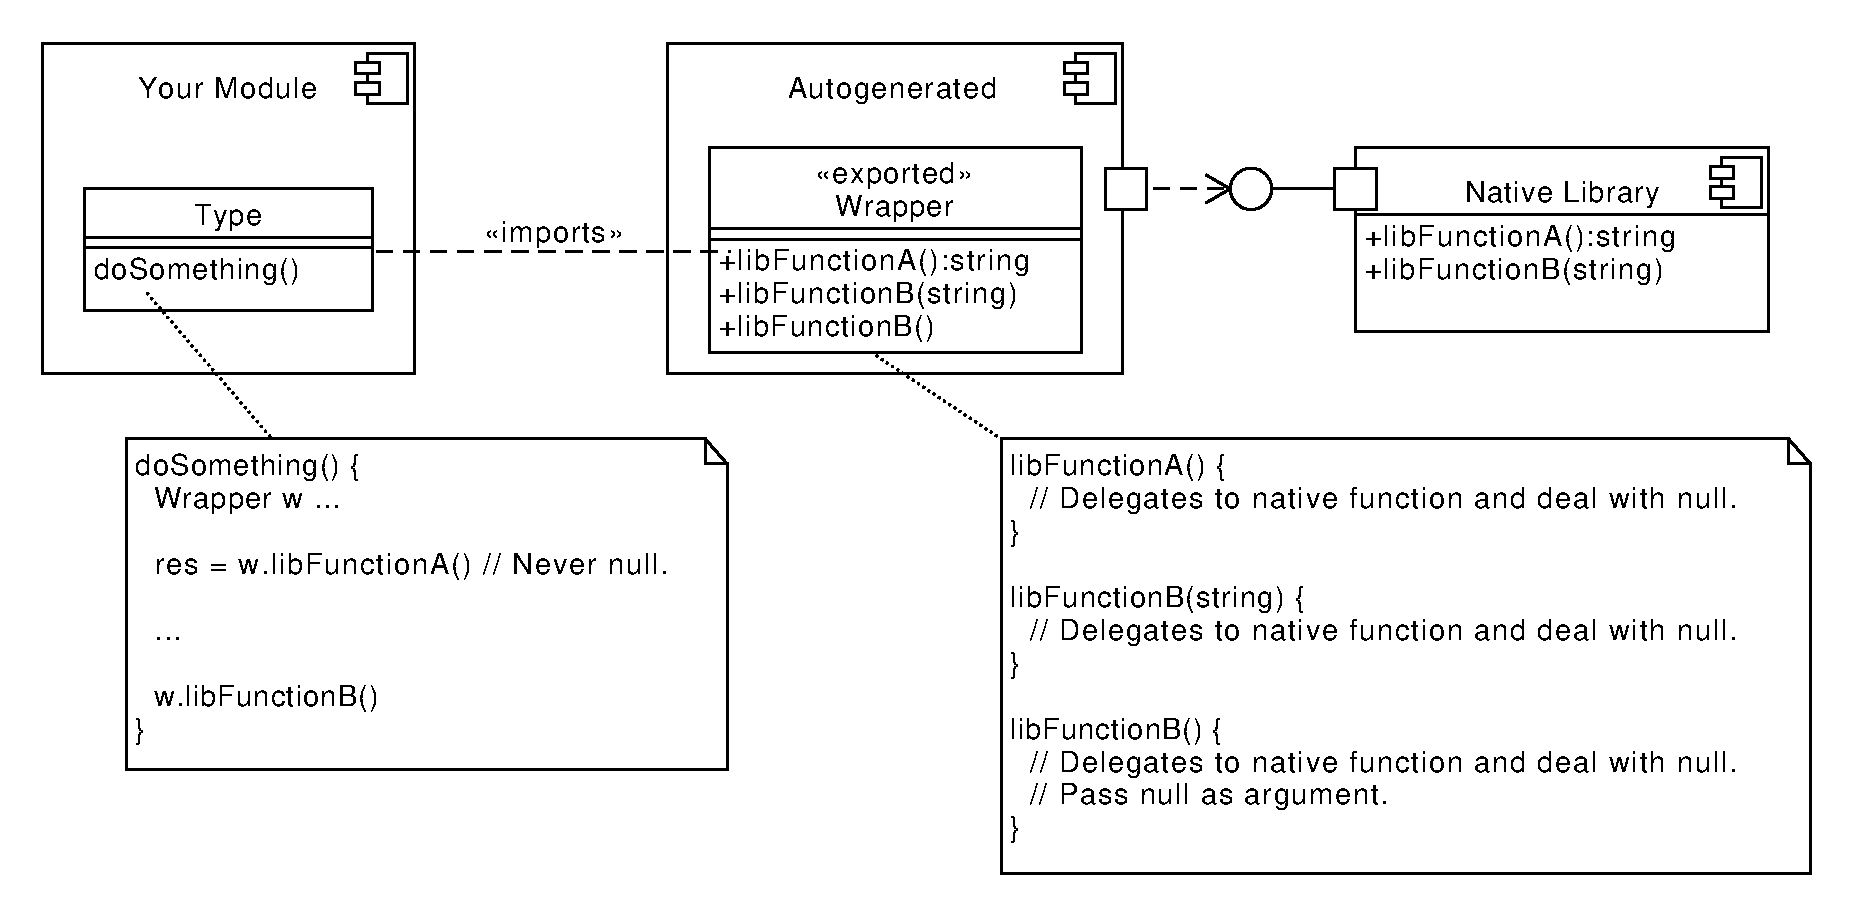
\includegraphics[width=350pt]{grafics/Generated_wrapper_for_linked_native_libs.pdf}
    \caption{Auto generated wrapper which deals with \textit{null} from linked native library (e.g.\ a C library)}
    \label{fig:Generated_wrapper_for_linked_native_libs}
\end{figure}

\subsection{Checked Exceptions}

\todo{Words from Andre Heilsberg (C\#)}

\subsection{Exceptions at All}

\todo{They are like goto (Javaslang)}

\subsection{Compiler or Interpreter Warnings}

Most languages (no matter if thy are compiled or interpreted) have some kind of warnings. The intention of these warnings is to tell the developer that he maybe did something wrong and should really reconsider the code. In the most cases the warnings are legit and the affected code should be changed to remove the warning to avoid bugs.

The fact about warnings is in my experience that they almost always are ignored. A lot of languages just do not display them by default. For example in PHP\footnote{\url{http://php.net/manual/en/function.error-reporting.php}} notices are not reported by default. So you get no message when you use a not existing array index or variable which may introduce subtle bugs. Despite that you can completely disable any reporting about errors. The same counts for Java: By default the compiler does not report warnings. This is the same story for pretty much every language. 

So what is the sense of warnings when they are ignored widely? In my opinion no sense! Either you did it right in your code or you did not. The compiler/interpreter should either stop with an error which tells you what you did not right or it should shut up because it is legit what the developer did. So in a modern high level language there should not be something like suppressible warnings. There should only be errors which stops the compilation/interpretation at all. So that developers can not ignore them.

\subsection{Goto}

Some languages offers a keyword named \texttt{goto}. The intention of it is to provide a way to jump away from the current code location to some other location (identified by line number or a named label depending on the languages implementation). To jump around in your code is a quite natural thing if you do Assembler or machine code because there you do not have high level control structures. E.g. a simple if-statement in machine code is done by testing a register for a certain condition and depending on the result either continue the execution or jump over some instructions to continue at an other point in the program.

Kernighan and Ritchie say about \textit{goto} in the book \textit{The C Programming Language}\cite{c-programming-lang}:

\begin{quotation}
    C provides the infinitely-abusable goto statement, and labels to branch to. Formally, the goto is never necessary, and in practice it is almost always easy to write code without it. We have not used goto in this book.
    Nevertheless, there are a few situations where gotos may find place. The most common is to abandon processing in some deeply nested structure, such as breaking out of two or more loops at once. The break statement cannot be used directly since it only exits from the inner loop.
\end{quotation}

So this is very clear: The \textit{goto} statement introduce a great chance to abuse it. And this is what most developers saw when thy stumbled upon \textit{goto} in production code. This is why nowadays \textit{goto} is considered a bad practice. Because it makes the code very hard to read, if the control flow jumps wildly around in the source code.

The reason Kernighan and Ritchie describes for when to use \textit{goto} seems to be legit. The provide an example in their book\cite{c-programming-lang}:

\begin{lstlisting}[language=C]
    for ( ... ) {
        for ( ... ) {
            ...
            if (disaster) {
                goto error;
            }
        }
    }
    
    error:
        clena up the mess
\end{lstlisting}

One may argue that they are completely right and one need \textit{goto} to do some error recovery like that. But also nowadays code like that is considered bad practice too. Because it has a way to high Cyclomatic complexity\footnote{\url{https://en.wikipedia.org/wiki/Cyclomatic_complexity}}. This means you should not use deeply nested control structures like in the example above because it makes the code less testable, robust and reusable.

So there is absolute no reason to add a feature like \textit{goto} to a modern high level language.

\section{Disappointing}

In this section I describe things which are very disappointing, e.g.\ typing boiler plate code, parens, semicolons and such. In contrast to the section before these points are merely opinion based. But I try to show why we should think about it.

\subsection{Unnecessary Braces in Coanditionals}

In lot of languages it is necessary to encapsulate conditionals in control structures with braces. The examples below are written in Java, but it is the same in C/C++/C\#/Objective-C/PHP/JavaScript etc. pp. Let's look into the most common control structures:

\begin{lstlisting}[language=Java]
    if (a > 0 && b < 10) { ... }
    
    for (String s : stringCollection) { ... }
    
    for (int i = 0; i < 10; ++i) { ... }
    
    switch (a) { ... }
    
    while (a < 10) { ... }
\end{lstlisting}

The common pattern is always

\begin{lstlisting}
    CONTROL-KEYWORD ( <<condition>> ) { 
        <<statements>> 
    }
\end{lstlisting}

The only exception to this are control structures with only one statement. In most languages then the curly braces are optional. Nowadays this is strongly considered as bad practice because it introduce the possibility of bugs: Someone adds a second line but forget the curly braces to group them as a block. So this feature should not be added to a new programming language. The argument that it requires more memory and space on the screen is obsolete nowadays.

Also most languages allow to have no space after the \textit{control keyword}

\begin{lstlisting}[language=Java]
    if(a > 0 && b < 10) { ... }
\end{lstlisting}

But this is also in most communities considered a bad practice. It does not increase the readability. So if we define that there must always be at last one  space after the keyword and the curly braces to group the statements together  then we can remove the braces to group the condition:

\begin{lstlisting}
    CONTROL-KEYWORD <<condition>> { 
        <<statements>> 
    }
\end{lstlisting}

A parser will consider the keyword as token, skips the next white space, and then recognize everything up to the open curly brace as conditional expression.

\subsection{Unnecessary Semicolon}

\todo{Read \url{https://en.wikipedia.org/wiki/Semicolon\#Programming} and \url{http://se.ethz.ch/\~meyer/publications/hoare/evolution.pdf}}

One of the most superfluous things in programming languages is the semicolon necessary to terminate a statement. The only reason for this was in former time when some engineers decided it will be a good idea to put more than one statement into a line\footnote{Allegedly it was first introduced by ALGOL 60 (\url{https://en.wikipedia.org/wiki/ALGOL_60}).}. The necessity for that were the small sized screens from that former time. They only had twenty-five lines but eighty columns. So it seemed to be a good idea. But nowadays it is common sense that it is not a good idea to put more than one statement in a line for readability and understanding of code. So from a parser perspective it is totally unnecessary to delimit statements with a special character unless you put more than one statement in each line. A lot of languages show that semicolons are not necessary to delimit statements: Ruby, Python, Go, Swift etc. But some of these language allow to delimit statements to be terminated with a semicolon. So you can put more than one statement into a line. But as mentioned this is nowadays not considered a good practice. Instead of allowing this for some really rare circumstances where it would be helpful it is better to not add this feature at all to circumvent abuse of this feature.

\subsection{Special Character Methods or Operators}

Each programming language provides some special symbols. Usually the operators are such. E.g.\ for math operations there are operators such as \texttt{+}, \texttt{-}, \texttt{*}, \texttt{/}. There is no problem with such simple operators. The problem arises when the language provides a mass of special kind operators a novice programmer is not used to.

Looking at Perl or Scala as a beginner you will notice a lot of strange characters in the code. Some examples from Perl\cite{secret-perl-operators}:

\begin{itemize}
    \item Spaceship operator: \texttt{<=>}
    \item Eskimo Greeting operator: \texttt{}{}
    \item Goatse operator: \texttt{=()=}
    \item Turtle operator: \texttt{@{[]}}
    \item Inchworm operator: \texttt{~~}
    \item Inchworm-On-A-Stick Operator: \texttt{~-}
    \item Spacestation Operator: \texttt{-+-}
    \item Venus operator: \texttt{0+}
\end{itemize}

Perl is an ancient language and we may argue that in former time this was a good idee to save space or typing, but modern languages also have this problem. Here some examples from Scala\cite{special-operators-scala}:

\begin{itemize}
    \item Upper, lower and view bounds: \texttt{<: >: <\%}
    \item Vararg expansion: \texttt{\_*|}
    \item Many different meanings: \texttt{\_}
\end{itemize}

I don't want to blame Perl or Scala in particular here. Other languages does this also: Haskell, Ruby etc. Especially functional languages tend to strange characters to name functions, methods or operators. In my opinion this violates the rule that source code should be least astonishing. Of course for a professional developer this may be time saving to type three characters instead of a long function name. This argument counted decades ago when the developers only had dumb text editors and small sized screens. Today we all have super power driven editors or IDEs with intellisense and auto completion and large scaled screens. So there is no reason to confuse developers without years of experience with strange characters.

I would also go even further: Some operators we are used to in almost every language should be reconsidered:

\begin{itemize}
    \item \textbf{Negation}: Most languages use the \texttt{!} to negate an expression. But this small character is often overseen. For example for a code fragment like \texttt{if (!foo) ...} it is very easy to oversee the not operator and remove it accidentally when refactotring the code. Some software projects state the rule that a condition like that must be written as \texttt{if (!!!foo) ...} or \texttt{if (false == foo) ...} to make the negation more obvious. This could be circumvented by replacing the \texttt{!} operator completely by a keyword \texttt{not}: \texttt{if (not foo) ...}. Some languages provide both possibilities, but I would strongly recommend only one way to not confuse novice programmers what to use. Also the idea of the control structucre \texttt{unless (foo) ...} instead of \texttt{if (not foo) ...} should be considered.
    \item \textbf{Logical Operators}: Most languages provide operators for boolean operations (e.g. \texttt{\&\&}, \texttt{||}) for logical \textit{and} and \textit{or}. The operator for \texttt{exclusive or} are more various over languages. Here it would be easier to provide also keywords: \texttt{and}, \texttt{or}, and \texttt{xor}.
\end{itemize}

\subsection{Language Tool Chain}

A lot of languages lack of appropriate tooling and it is necessary to build them first before you get productive. A perfect language must come with all necessary tools: a \textit{language tool chain}. What are necessary tools which should be provided by such a tool chain?

All languages have at least a compiler or interpreter. And mostly that is all you get. But to be productive to create more than simple small applications a developer (team) need tools for

\begin{itemize}
    \item compile and link all sources to a usable self contained\footnote{In my opinion everything should be self contained so you circumvent the problem that final artifacts require libraries in different versions. Each artifact comes with all its dependencies. This will consume more disk space, but this is not an issue anymore.} binary or library.
    \item manage dependencies so that they do not interfere with each other when they have same modules in different versions as transitive dependency.
    \item executes test code (unit, integration, and system tests) and report code coverage.
    \item source code formatting and linting.
    \item create API documentation for a module.
\end{itemize}

The Go\footnote{\url{https://golang.org/doc/cmd}} programming language is a good example for that. It provided from start a comprehensive tool chain to maintain the above mentioned tasks. One negative example is Java where you have to compile all your classes by self and put all dependencies on the classpath etc. pp., unless you use tools like Maven\footnote{\url{https://maven.apache.org/}} or Ant\footnote{\url{http://ant.apache.org/}}. But botch of these tools came years after the first release of Java. That's a reason why you can find nowadays software projects which only builds in a particular IDE on a particular system. When talking to the developers they always say: ``We never heard about Maven/Ant etc.'' There are also other examples: For C you need to now about \textit{make}. But there exists different flavours/implementation of make (GNU make\footnote{\url{https://www.gnu.org/software/make/}}, CMake\footnote{\url{https://cmake.org/}}, DMake\footnote{\url{https://www.openoffice.org/tools/dmake/}} etc.) and of course they are not full compatible. If all necessary tools are provided by the language itself with sane defaults and specification, then there is not the problem that every project has its own build mechanics incompatible to each other. Also you loose the necessity to discuss how to do it with everybody. Remember how long you discussed the last time in a team how to configure the code formatter. Easy solution: The language ships one code formatter with only one sane default format: No discussions about tabs versus spaces or such anymore.

\section{Other Disadvantages}

\subsection{Inheritance}

On of the very first concepts you learn when starting with \textit{object oriented programming (OOP} is \textit{inheritance}. Typically you will be introduced to the concept of \textit{OOP} by describing your problem domain in the programming language like real world objects. There will come up an example like: You have dog objects and cat objects. They have properties and behaviour in common and some properties and behaviour which distinguishes them. The parts which are common will be represented as properties and behaviour of a common parent class (Figure ~\ref{fig:Classical_inheritance_example}).

\begin{figure}[ht]
    \centering
    \includegraphics[width=350pt]{grafics/Classical_inheritance_example.pdf}
    \caption{Example of a classical inheritance.}
    \label{fig:Classical_inheritance_example}
\end{figure}

This is a very helpful example, if you have to write a software for a vet or zoo. In most software only a small part can be modelled like this. Usually this is the domain model. A lot of more code you will have for all the other stuff which makes you software run: There must be classes for file operations, for the user interface, for network operations, for user authentication etc. pp. How to model this like real world objects? That's quite bit more difficult than the animal example. In theory you should look at all these classes and model them accordingly to the animal example: Common property and behaviour should be extracted in a parent class. But in fact you will see a lot inheritance only to get access to a functionality of another object. To give an example suitable to the above animals: You add the property that a dog have four legs. Later someone would say that cats also have four legs and pulls up that property to the animal type. But then you have to add some snakes and birds to your domain model. Both of them does not have four legs. The snake has no legs and birds have two of them. So lets introduce some more types (Figure ~\ref{fig:Classical_inheritance_with_more_parents}). One may say that the numbers of legs should be a property in the animal class. That would be of course the better design, but here it to demonstrate the generel principle behind inheritance and the danger of creating overly complex inheritance trees. 

\begin{figure}[ht]
    \centering
    \includegraphics[width=350pt]{grafics/Classical_inheritance_with_more_parents.pdf}
    \caption{A slightly more complex inheritance example.}
    \label{fig:Classical_inheritance_with_more_parents}
\end{figure}

So what is the problem with inheritance and why do some state that \textit{composition should be favoured over inheritance}? One of the problems is that inheritance exposes a subclass to details of its parent's implementation and so breaks encapsulation\cite{gang-of-four}. This would make the software less testable and robust and also may introduce subtle bugs (e.g.\ overridable method call in constructor). Another problem is that for a good designed model with inheritance it should respect the \textit{Liskov substitution principle}\footnote{\url{https://en.wikipedia.org/wiki/Liskov_substitution_principle}}. Which simply says that whenever you can pass a animal type (from above example) into a method, then this method must work correct also if you pass in a dog or cat. This is often not the case in software systems when inheritance is used only to obtain some functionality from another class. The typical case of: There is a function which does exactly what I want, but copy and paste is evil, so lets extend that class. How difficult it is to do this correctly is mentioned in an excellent article\footnote{\url{http://www.artima.com/lejava/articles/equality.html}} about how to implement the \texttt{Object\#equals(Object)} right in Java for subclasses. Also problematic is the fact that inheritance in most languages is done at compile time. If you want to give the dog in the example above another parent class, then you must recompile and redeploy the software. In most languages there is no chance to change a parent class at runtime (which is necessary to enable static type checking at compile time). And last but not least there is multiple inheritance. Most languages does not allow it to circumvent the \texttt{Diamond problem}\footnote{\url{https://en.wikipedia.org/wiki/Multiple_inheritance\#The_diamond_problem}}. In such languages you will be faced with the problem that your domain model requires multiple inheritance, but you have to workaround it to fit into the single inheritance. All this leads to unnecessary complex code and boiler plate code.

In contrast composition bypass these problems. With composition our animal example will look like different: The dog and animal class will have a property holding an instance of an animal object and delegates the all method calls to it (Figure ~\ref{fig:Composition_example}). With this approach you have not to leak the internals of the common animal class into the subclasses and therefore you need not to break the encapsulation. Also you may change the animal class at runtime. This makes code often more testable because you can inject a mock implementation of the animal type. Also it provides a easy solution to the \textit{Diamond problem}: You can declare as many delegates you want, but you decide which methods to use of them. If you have two delegates with the same method and you need both of them you can just rename the delegate method for one or both of them.

\begin{figure}[ht]
    \centering
    \includegraphics[width=350pt]{grafics/Composition_example.pdf}
    \caption{Now the same example with composition instead of inheritacne.}
    \label{fig:Composition_example}
\end{figure}

The major downside of this delegation in most languages is that you need to write lot of boilerplate code. For example in Java the animal example will look like:

\begin{lstlisting}[language=Java]
    class Animal {
        void eat() { ... }
        void sleep() { ... }
    }
    
    class Dog {
        private Animal delegate = new Animal();
        
        void eat() { delegate.eat(); }
        void sleep() { delegate.sleep(); }
        void retrieve() { ... }
    }
    
    class Cat {
        private Animal delegate = new Animal();
    
        void eat() { delegate.eat(); }
        void sleep() { delegate.sleep(); }
        void playWithBallOfWool() { ... }
    }
\end{lstlisting}

Most modern IDEs support the developer by auto generating such boiler plate code. But nevertheless it clutters up the code. In a modern \textit{OOP} language it would be nice to let the compiler do this for you. So there should be language constructs to support such composition, e.g.

\begin{lstlisting}
    class Animal {
        void eat() { ... }
        void sleep() { ... }
    }
    
    class Dog {
        delegate Animal;
        
        void retrieve() { ... }
    }
    
    class Cat {
        delegate Animal;
    
        void playWithBallOfWool() { ... }
    }
\end{lstlisting}

Obviously this implies that a common type like the animal in the above examples must not be abstract. In consequence if a feature like inheritance is completely removed fro the feature set of a language such abstract classes are not necessary. In classical \textit{OOP} you may want to prohibit one from creating an animal object because it make no sense to have such an object. But in a composition style it makes total sense.

\subsection{Visibility}

Most languages in the \textit{OOP} have the feature to declare the visibility of certain pars (namely the properties, methods and types). The general rule of \textit{OOP} is to hide as much of the implementation details as possible. But the problem with most language implementation is that the defaults are way to weak. So for example in Java the default visibility (if you give the compiler no hint) is package private, which means that everything else in the same package may access it. This is then exacerbated by various IDEs which mostly have the default to mark everything public which is auto generated, unless you change your default. Most novice programmer do not do this and thus produce way to public APIs. The problem with that is that this leads to tangled call which violates layers and abstractions. And the problem is that making things less visible later on is very difficult, unless you want to break existing code.\todo{Add reference to \url{https://martinfowler.com/ieeeSoftware/published.pdf}}

\subsubsection{Properties}

By default properties should always be private. There is no reason to expose them outside of the type, unless to violate the encapsulation and information hiding principle of \textit{OOP}. But sometimes you need to read or write such a property from outside. Typically you introduce setter and getter methods for your property. But this also clutters up your code. For example in Java you would write:

\begin{lstlisting}[language=Java]
    class Type {
        private String peropertyOne;
        private String peropertyTwo;
        private String peropertyThree;
        ...
        
        String getPropertyOne() {
            return propertyOne;
        }
        
        void setPropertyOne(String newPropertyOne) {
            propertyOne = newPropertyOne;
        }
        
        String getPropertyTwo() {
            return propertyTwo;
        }
        
        void setPropertyTwo(String newPropertyTwo) {
            propertyTwo = newPropertyTwo;
        }
        
        String getPropertyThree() {
            return propertyThree;
        }
        
        void setPropertyThree(String newPropertyThree) {
            propertyThree = newPropertyThree;
        }
        
        ...
    }
\end{lstlisting}

Without a vast amount of self discipline this will not work out well. Wouldn't it be nicer to let the compiler auto generate such getters and setters?

\begin{lstlisting}
    class Type {
        property String peropertyOne;
        property String peropertyTwo;
        property String peropertyThree;
    }
\end{lstlisting}

This woul lead into much cleaner code and less work for developers. But there must be some modifiers to tell whether such propert is readable or writable:

\begin{lstlisting}
    class Type {
        property(read) String peropertyOne;
        property(read, write) String peropertyTwo;
        property(write) String peropertyThree;
    }
\end{lstlisting}

\todo{Find examples which does this already (Objective-C, C\#, Swift?).}
    
\subsubsection{Methods}

In contrast to properties methods sometimes should be more visible than private because a object which only have private methods will not be very useful. But the above mentioned points about the defaults also holds here. For example in Java by default methods are package private and most IDEs generate new method stubs public. This will lead to the same problems. So in a modern programming language the default visibility for methods should always be private and only if the developer decides it would be a good idea the visibility must be opened explicit by a keyword.

Most languages provide four levels of visibilities for methods:

\begin{description}
    \item[private] The method is only accessible from within the same type which declares that method.
    \item[package private] Only objects which type is declared in the same package as the type declaring the method can access that method.
    \item[protected] Every type which extends this type can access a protected method from that parent.\footnote{In a language which does not have inheritance, but a delegation model (as described above) may not need this level of visibility.}
    \item[public] Every other object can access a public method.
\end{description}

The problem arises with the \textit{public} level because in most languages public methods are also accessible from other modules. Fowler calls this published API\todo{Reference to Article about published interfaces.}. Sometimes your design requires to open the visibility of methods to \textit{public} so that you can call them from another package, but you do not want that some client code which uses your module calls it. The only way you have in e.g.\ in Java is to document that in your method documentation that nobody should use that method. Problem is nobody will read that. A solution would be to add one more level to mark methods that they are \textit{exported} so that \textit{public} methods are not automatically published into the wild.

\subsubsection{Types}

For types also the same holds as for methods described above. But the default visibility of a type must not be \textit{private} because such type would be quite useless because no other code could use it. Instead of a sane default is \textit{package private} and a type must be explicitly marked \textit{public}. Also it would be useful to have the additional level to export a type like described for methods.

One aspect of the \textit{package private} level should be reconsidered: In most languages \textit{package private} means that only types from within the same package (which merely means same directory). But lets imagine an example where you have a library which provides some serializers: You have a factory which creates them (example in Java):

\begin{lstlisting}[language=Java]
    public interface Serliazer { ... }
    
    public class Factory {
        public Serliazer createFoo() { 
            return new FooSerliazer();
        }
        
        public Serliazer createBar() { 
            return new BarSerliazer();
        }
    }    
    
    FooSerliazer implements Serliazer { ... }

    BarSerliazer implements Serliazer { ... }
\end{lstlisting}

Of course you want to make the implementations package private so that only the factory can create instances. All other types in your module or client code from other modules must use the factory. In Java and lot of other languages this works fine as long as all types are in the same package. But if the implementations of the concrete serializers become more complex and have more own types incorporated you would put them in own sub packages like:
\\
\dirtree{%
.1 serializer.
.2 Serliazer.
.2 Factory.
.2 foo.
.3 FooSerliazer.
.3 \dots.
.2 bar.
.3 BarSerliazer.
.3 \dots.
}

To get this work in Java you must make the implementations (\texttt{FooSerliazer} and \texttt{BarSerliazer} public, unless the Factory can not access them. This introduces the risk that a consumer of that API may also use these types directly which is highly undesired. A solution may be that \textit{package private} also works for sub packages. Means in the above example that everything in the package \texttt{serializer} can see anything which is \textit{package private} in its subpackages. A point to discuss further: If this is only possible from top down in the package hierarchy (which is essential for the above problem) or should it also work from bottom up (should the subpackages also see anything \textit{package private}) from its superordinated packages). Definitely it must be prohibited to see \textit{package private} from sibling packes (everything inside the package \texttt{foo} must not see anything from package \texttt{bar}, unless it is \textit{public}.

\subsection{Static}

\todo{Should not be used in OOP. Introduces the risk of static methods with side effects. Instead of static members introduce a const keyword.}

\chapter{Good Ideas Out There}

In this section interesting ideas and concepts of already existing languages will be described and considered if they are worth and useful for a new modern programming language.

\section{Multiple Return}

\todo{Write about multiple return.}

\section{Defaults for Arguments}

\todo{Write about defaults for arguments.}

\section{Named Arguments}

\todo{Write about named arguments.}

\section{Multiple Dispatch}

\todo{Write about multiple dispatch.}

\section{Dependent Types}

\todo{Write about dependent types.}

\section{Pattern Matching}

\todo{Write about pattern matching.}

\chapter{TODO -- Ideas}

\section{Kotlin}

From a blog post from Peter Sommerhoff\cite{kotlin-sommerhoff}:

\subsection{Data Classes}

Simple POJOs are declared simpler. Instead of writing boiler plate like:

\begin{lstlisting}
class Book {
    private String title;
    private Author author;

    public String getTitle() {
        return title;
    }
    
    public void setTitle(String title) {
        this.title = title;
    }

    public Author getAuthor() {
        return author;
    }
    
    public void setAuthor(Author author) {
        this.author = author;
    }
}
\end{lstlisting}

You can write:

\begin{lstlisting}
data class Book(var title: String, var author: Author) {
    // ...
}
\end{lstlisting}

\subsection{Smart Casts}

Instead of:

\begin{lstlisting}
if (node instanceof Leaf) {
    return ((Leaf) node).symbol;
}
\end{lstlisting}

less verbose:

\begin{lstlisting}
if (node is Leaf) {
    return node.symbol;
}
\end{lstlisting}

\subsection{Type Inference}
\todo{Write text for type inference.}

\subsection{Functional Programming}
\todo{Write text for functional programming.}

\subsection{Default Arguments}
\todo{Write text for default arguments.}

\subsection{Named Arguments}
\todo{Write text for named assignments.}

\subsection{Final Classes}

\begin{quotation}
Next, Kotlin also supports the principle to either design for inheritance or prohibit it — because in Kotlin, you have to explicitly declare a class as open in order to inherit from it. That way, you have to remember to allow inheritance instead of having to remember to disallow it.\cite{kotlin-sommerhoff}
\end{quotation}

\listoffigures

\begin{thebibliography}{100}
	
\bibitem{null-wiki}
    Wikipedia,
    \emph{Null pointer},
    \url{https://en.wikipedia.org/wiki/Null_pointer}

\bibitem{kent-dyn-err-remediation}
    Stephen W. Kent,
    \textit{Dynamic Error Remediation: A Case Study with Null Pointer Exceptions},
    \url{http://citeseerx.ist.psu.edu/viewdoc/download?doi=10.1.1.140.2544&rep=rep1&type=pdf}

\bibitem{hoare-wiki}
    Wikipedia,
    \textit{Tony Hoare},
    \url{https://en.wikipedia.org/wiki/Tony_Hoare}
    
\bibitem{hoeare-null}
    Tony Hoare,
    \textit{Speaking at a conference in 2009},
    \url{http://www.infoq.com/presentations/Null-References-The-Billion-Dollar-Mistake-Tony-Hoare}

\bibitem{draper-worst-mistake-cs}
    Paul Draper,
    \textit{The worst mistake of computer science},
    \url{https://www.lucidchart.com/techblog/2015/08/31/the-worst-mistake-of-computer-science/}

\bibitem{kotlin-sommerhoff}
 	Peter Sommerhoff,
 	\textit{Kotlin for Java Developers: 10 Features You Will Love About Kotlin},
 	\url{https://www.javacodegeeks.com/2016/05/kotlin-java-developers-10-features-will-love-kotlin.html}

\bibitem{secret-perl-operators}
    Peteris Krumin,
    \textit{Secret Perl Operators},
    \url{http://www.catonmat.net/blog/secret-perl-operators/}

\bibitem{special-operators-scala}
    Daniel C. Sobral,
    \textit{What do all of Scala's symbolic operators mean?},
    \url{http://stackoverflow.com/questions/7888944/what-do-all-of-scalas-symbolic-operators-mean}
    
\bibitem{murphys-law}
    Wikipedia,
    \textit{Murphy's law},
    \url{https://en.wikipedia.org/wiki/Murphy's_law}

\bibitem{golang-spec}
    Go Programming Language,
    \textit{The Go Programming Language Specification},
    \url{https://golang.org/ref/spec}

\bibitem{swift-spec-optional-chaining}
    The Swift Programming Language,
    \textit{Optional Chaining},
    \url{https://developer.apple.com/library/content/documentation/Swift/Conceptual/Swift_Programming_Language/OptionalChaining.html}
    
\bibitem{null-in-fsharp}
    F\# Language Reference,
    \textit{This topic describes how the null value is used in F\#},
    \url{https://docs.microsoft.com/en-us/dotnet/articles/fsharp/language-reference/values/null-values}.

\bibitem{optional-in-fsharp}
    F\# Language Reference,
    \textit{Options},
    \url{https://docs.microsoft.com/en-us/dotnet/articles/fsharp/language-reference/options}

\bibitem{c-programming-lang}
    The C Programming Language (2nd Edition),
    \textit{Brian W. Kernighan, Dennis M. Ritchie},
    Prentice Hall Software Series, 1988

\bibitem{gang-of-four}
    Design Patterns: Elements of Reusable Object-Oriented Software,
    \textit{Erich Gamma, Richard Helm, Ralph Johnson, John Vlissides},
    Prentice Hall, 1994

\end{thebibliography}

\end{document}
